%\documentclass[12pt,draftcls]{ucdavisthesis}
\documentclass[12pt]{ucdavisthesis}

% PLEASE READ THE MANUAL - ucdavisthesis.pdf (in the package installation directory)

%%%%%%%%%%%%%%%%%%%%%%%%%%%%%%%%%%%%%%%%%%%%%%%%%%%%%%%%%%%%%%%%%%%%%%%%
%                                                                      %
%               LATEX COMMANDS FOR DOCUMENT SETUP                      %
%                                                                      %
%%%%%%%%%%%%%%%%%%%%%%%%%%%%%%%%%%%%%%%%%%%%%%%%%%%%%%%%%%%%%%%%%%%%%%%%

%\usepackage{bookmark}
\usepackage[us,nodayofweek,12hr]{datetime}
\usepackage{graphicx}
%\usepackage[square,comma,numbers,sort&compress]{natbib}
%\usepackage{hypernat}
% Other useful packages to try
%\usepackage{amsmath}
%\usepackage{amssymb}
%
% Different fonts to try (uncomment only fontenc and one font at a time)
% (you may need to install these first)
%\usepackage[T1]{fontenc} %enable fontenc package if using one of the fonts below
%\usepackage[adobe-utopia]{mathdesign}
%\usepackage{tgschola}
%\usepackage{tgbonum}
%\usepackage{tgpagella}
%\usepackage{tgtermes}
%\usepackage{fourier}
%\usepackage{fouriernc}
%\usepackage{kmath,kerkis}
%\usepackage{kpfonts}
%\usepackage[urw-garamond]{mathdesign}
%\usepackage[bitstream-charter]{mathdesign}
%\usepackage[sc]{mathpazo}
%\usepackage{mathptmx}
%\usepackage[varg]{txfonts}

\hyphenation{dis-ser-ta-tion blue-print man-u-script pre-par-ing} %add hyphenation rules for words TeX doesn't know


%\renewcommand{\rightmark}{\scriptsize A University of California Davis\ldots \hfill Rev.~\#1.0 \quad Compiled: \currenttime, \today}
% a fancier running header that can be used with draftcls options

%%%%%%%%%%%%%%%%%%%%%%%%%%%%%%%%%%%%%%%%%%%%%%%%%%%%%%%%%%%%%%%%%%%%%%%%
%                                                                      %
%        DOCUMENT SETUP AND INFORMATION FOR PRELIMINARY PAGES          %
%                                                                      %
%%%%%%%%%%%%%%%%%%%%%%%%%%%%%%%%%%%%%%%%%%%%%%%%%%%%%%%%%%%%%%%%%%%%%%%%

\title          {A Polyhedral Finite Element Approach to \\ 
                 Image-Based Modeling and Simulation in Biomechanics}
%Exact title of your thesis. Indicate italics where necessary by underlining or using italics. Please capitalize the first letter of each word that would normally be capitalized in a title.

\author         {Omar Mohamed Hafez}
%Your full name as it appears on University records. Do not use initials.

\authordegrees  {B.S. Civil Engineering (University of California, Davis) 2009 \\
                 M.S. Civil Engineering (University of California, Davis) 2010 \\
                 M.S. Applied Mathematics (University of California, Davis) 2012}
%Indicate your previous degrees conferred.

\officialmajor  {CIVIL AND ENVIRONMENTAL ENGINEERING}
%This is your official major as it appears on your University records.

\graduateprogram{Civil and Environmental Engineering}
%This is your official graduate program name. Used for UMI abstract.

\degreeyear     {2017}
% Indicate the year in which your degree will be officially conferred.

\degreemonth    {December}
% Indicate the month in which your degree will be officially conferred. Used for UMI abstract.

\committee{Mark Rashid}{Committee Member Name}{Committee Member Name}{}{}
% These are your committee members. The command accepts up to five committee members so be sure to have five sets of braces, even if there are empties.

%%%%%%%%%%%%%%%%%%%%%%%%%%%%%%%%%%%%%%%%%%%%%%%%%%%%%%%%%%%%%%%%%%%%%%%%

%\copyrightyear{2017}
%\nocopyright

%%%%%%%%%%%%%%%%%%%%%%%%%%%%%%%%%%%%%%%%%%%%%%%%%%%%%%%%%%%%%%%%%%%%%%%%

\dedication{\textsl{To \ldots}}

%%%%%%%%%%%%%%%%%%%%%%%%%%%%%%%%%%%%%%%%%%%%%%%%%%%%%%%%%%%%%%%%%%%%%%%%

\abstract{The abstract submitted as part of your dissertation, in the introductory pages, does not have a word limit. It should follow the same format as the rest of your dissertation (1.5 inch left margin, double-spaced, consecutive page numbering, etc.).}

%%%%%%%%%%%%%%%%%%%%%%%%%%%%%%%%%%%%%%%%%%%%%%%%%%%%%%%%%%%%%%%%%%%%%%%%

\acknowledgments{Acknowledgements to those who helped you get to this point. They should be listed by chapter when appropriate.}

%%%%%%%%%%%%%%%%%%%%%%%%%%%%%%%%%%%%%%%%%%%%%%%%%%%%%%%%%%%%%%%%%%%%%%%%

% Each chapter can be in its own file for easier editing and brought in with the \include command.
% Then use the \includeonly command to speed compilation when working on a particular chapter.
%%% \includeonly{chap1}

\begin{document}

\newcommand{\bibfont}{\singlespacing}
% need this command to keep single spacing in the bibliography when using natbib

\bibliographystyle{ieeetr}
%many other bibliography styles are available (IEEEtran, mla, etc.). Use one appropriate for your field.

\makeintropages %Processes/produces the preliminary pages

\chapter{Overview}
%

\textit{Image-based modeling and simulation}, also known as \textit{patient-specific modeling and simulation} or \textit{in-silico modeling and simulation}, is the process of performing computations based on imaging data to analyze and predict the physical behavior of biological tissues.

benefits

possibilities

FDA
VV40?

cite everyone doing it

Image-based modeling and simulation covers a broad spectrum of fields, including image processing, computational geometry, numerical methods, and biomechanics. The workflow entails: image processing and image segmentation, image-based mesh generation, physics-based modeling and simulation, and finally a 

Medical images will be assumed here to be 

nonlinear solid mechanics
finite element methods and their variants

For the electronic version of this document, images may be zoomed into for detail.

rectilinear grid of voxels, or three-dimensional pixels
\chapter{Medical Imaging}
%
\begin{figure}[tbh]
\centering
\includegraphics{media/ucdavisthesis_example_figure}
% where an .eps filename suffix will be assumed under latex,
% and a .pdf suffix will be assumed for pdflatex
\caption[First sample figure]{A sample figure.}
\label{fig.sample_1}
\end{figure}

\section{Magnetic Resonance Imaging}
\label{Magnetic Resonance Imaging}

MRI is ideal for visually distinguishing soft tissues, but objects MUST contain hydrogen molecules (e.g. water). However it is possible to get around this problem and scan “dry” objects made of plastic, for example, by immersing them in jelly. The negative of the object is then visible in the MRI data. Segmentation can be threshold based in some cases. Unfortunately it is quite common for different objects to be easily distinguishable visually, by texture, but not by greyscale. In these cases some level of manual segmentation may be required. MRI images often suffer from signal attenuation and/or noise on the borders of the region of interest. \\

MRI, CT, ultrasound, others \\

%%%%%%%%%%%%%%%%%%%%%%%%%%%%%%%%%%%%%%%%%%%%%%%
%%%%%%%%%%%%%%%%%%%%%%%%%%%%%%%%%%%%%%%%%%%%%%%
\subsection{Diffusion Tensor MRI}
\label{Diffusion Tensor MRI}

\section{Computed Tomography}
\label{Computed Tomography}
X-ray computed tomography (CT) $\rightarrow$ becoming more popular \\
%%%%%%%%%%%%%%%%%%%%%%%%%%%%%%%%%%%%%%%%%%%%%%%
%%%%%%%%%%%%%%%%%%%%%%%%%%%%%%%%%%%%%%%%%%%%%%%
\section{Other Imaging Technologies}
\label{Other Imaging Technologies}
Ultrasound (3D), Elastography, etc.
\chapter{Image Segmentation}
%

~\cite{morel} -- Mumford-Shah model\\
~\cite{mitiche}
threshold based segmentation
edge based
region based
clustering
matching

future - neural networks

%%%%%%%%%%%%%%%%%%%%%%%%%%%%%%%%%%%%%%%%%%%%%%%
%%%%%%%%%%%%%%%%%%%%%%%%%%%%%%%%%%%%%%%%%%%%%%%
\section{Review of Image Segmentation Techniques}
\label{Review of Image Segmentation Techniques}
%%%%%%%%%%%%%%%%%%%%%%%%%%%%%%%%%%%%%%%%%%%%%%%
%%%%%%%%%%%%%%%%%%%%%%%%%%%%%%%%%%%%%%%%%%%%%%%
\subsection{Level Sets}
\label{Level Sets}

%%%%%%%%%%%%%%%%%%%%%%
%%%%%%%%%%%%%%%%%%%%%%
\subsection{Flood Fill}
\label{Flood Fill}
%%%%%%%%%%%%%%%%%%%%%%
%%%%%%%%%%%%%%%%%%%%%%
\subsection{Color Space Voronoi Partitioning}
\label{Color Space Voronoi Partitioning}
~\cite{lcevt}
%%%%%%%%%%%%%%%%%%%%%%
%%%%%%%%%%%%%%%%%%%%%%
\subsection{Adaptive Template-Moderated}
\label{Adaptive Template-Moderated}
%%%%%%%%%%%%%%%%%%%%%%
%%%%%%%%%%%%%%%%%%%%%%
\subsection{Manual Approaches}
\label{Manual Approaches}
Seg3D, Simpleware, ITK-Snap \\
Invesalius


\chapter{Mesh Generation}
%

\begin{figure}[ht]
\centering
\subfigure[]{%
		
\includegraphics[scale=0.59]{media/2-shabaka/1-vor/dem1.png}
\label{fig:vor1}}
\subfigure[]{%
		\includegraphics[scale=0.59]{media/2-shabaka/1-vor/dem2.png}
\label{fig:vor2}}
\subfigure[]{%
		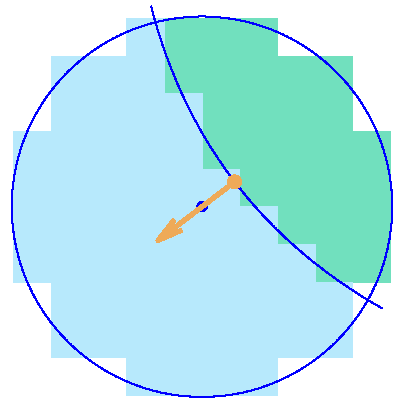
\includegraphics[scale=0.59]{media/2-shabaka/1-vor/dem3.png}
\label{fig:vor3}}
\subfigure[]{%
		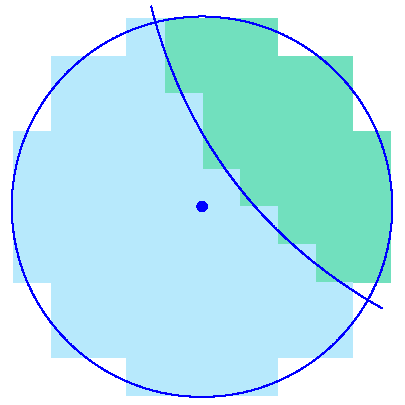
\includegraphics[scale=0.59]{media/2-shabaka/1-vor/dem4.png}
\label{fig:vor4}}
%
\caption{(a) Sample window of segmented image, (b) interface approximation, (c) point/normal placement, and d) Voronoi site placement}
\label{fig:vor}
\end{figure}

\begin{figure}[ht]
\centering
\subfigure[]{%
		\includegraphics[scale=0.085]{media/2-shabaka/3-clean-zoom/1-init-zoom.png}
\label{fig:cross1-1}}		
\subfigure[]{%
		\includegraphics[scale=0.085]{media/2-shabaka/3-clean-zoom/2-badfacets-zoom.png}
\label{fig:cross1-2}}		
\subfigure[]{%
		\includegraphics[scale=0.085]{media/2-shabaka/3-clean-zoom/3-badsegs-zoom.png}		
\label{fig:cross1-3}}					
\subfigure[]{%
		\includegraphics[scale=0.085]{media/2-shabaka/3-clean-zoom/4-fine-zoom.png}
\label{fig:cross1-4}}				
%
\caption{Clean-up of undesirable ``cross-talk'' facets for a surface patch: (a) initial surface following Voronoi-based surface reconstruction, (b) identification of ``cross-talk'' facets, (c) identification of edges to be collapsed, (d) final cleaned surface.}
\label{fig:cross1}
\end{figure}

\begin{figure}[ht]
\centering
\subfigure[]{%
		\includegraphics[scale=0.075]{media/2-shabaka/4-clean/1-init.png}
\label{fig:cross2-1}}		
\subfigure[]{%
		\includegraphics[scale=0.075]{media/2-shabaka/4-clean/2-badfacets.png}
\label{fig:cross2-2}}		
\subfigure[]{%
		\includegraphics[scale=0.075]{media/2-shabaka/4-clean/3-badsegs.png}	
\label{fig:cross2-3}}						
\subfigure[]{%
		\includegraphics[scale=0.075]{media/2-shabaka/4-clean/4-fine.png}		
\label{fig:cross2-4}}		
%
\caption{Clean-up of undesirable ``cross-talk'' facets for surface of \textit{ex-vivo} human heart: (a) initial surface following Voronoi-based surface reconstruction, (b) identification of ``cross-talk'' facets, (c) identification of edges to be collapsed, (d) final cleaned surface.}
\label{fig:cross2}
\end{figure}

\begin{figure}[ht!]
\centering
\subfigure[]{%
		\includegraphics[scale=0.1]{media/2-shabaka/2-surf/1-seg.png}
\label{fig:shabakaseq1}}
\subfigure[]{%
		\includegraphics[scale=0.1]{media/2-shabaka/2-surf/2-normals.png}
\label{fig:shabakaseq2}}
\subfigure[]{%
		\includegraphics[scale=0.1]{media/2-shabaka/2-surf/3-ptcloud.png}
\label{fig:shabakaseq3}}
\subfigure[]{%
		\includegraphics[scale=0.1]{media/2-shabaka/2-surf/4-finesurf.png}
\label{fig:shabakaseq4}}
\subfigure[]{%
		\includegraphics[scale=0.1]{media/2-shabaka/2-surf/5-surf.png}
\label{fig:shabakaseq5}}
%
\caption{(a) Segmented image, (b) point/normal placement, (c) oriented point cloud (normals not shown), c) cleaned surface mesh generated from Voronoi partition (edges not shown), and d) final decimated surface}
\label{fig:shabakaseq}
\end{figure}

\begin{figure}[ht!]
\centering
\vspace{2.5mm}
\includegraphics[width=1.0\textwidth]{media/2-shabaka/2-surf/6-showcase.png}
\caption{Suite of example surfaces generated from image data.}
\label{fig:showcase}
\end{figure}

\begin{figure}[ht!]
\centering
\vspace{2.5mm}
\includegraphics[width=1.0\textwidth]{media/2-shabaka/2-surf/7-shabaka.png}
\caption{Screenshot of Github repo}
\label{fig:github}
\end{figure}

\begin{figure}[ht]
\centering
\subfigure[]{%
		\includegraphics[scale=0.14]{media/4-cardioid/0-ventriclesurf.png}
\label{fig:tet1}}
\subfigure[]{%
		\includegraphics[scale=0.14]{media/4-cardioid/1-tet.png}
\label{fig:tet2}}
%
\caption{Bi-ventricular mesh: (a) surface mesh, and (b) clipped view of quadratic tetrahedral mesh used in Cardioid simulations}
\label{fig:tetmesh}
\end{figure}

\begin{figure}[ht]
\centering
\subfigure[]{%
		\includegraphics[scale=0.2]{media/3-celeris/1-brep.png}
\label{fig:cel1}}		
\subfigure[]{%
		\includegraphics[scale=0.2]{media/3-celeris/2-hex.png}
\label{fig:cel2}}		
\subfigure[]{%
		\includegraphics[scale=0.2]{media/3-celeris/3-pmesh.png}
\label{fig:cel3}}		
\subfigure[]{%
		\includegraphics[scale=0.2]{media/3-celeris/4-clip.png}
\label{fig:cel4}}	
\subfigure[]{%
		\includegraphics[scale=0.2]{media/3-celeris/5-color.png}
\label{fig:cel5}}			

\caption{Generation of polyhedral mesh: (a) input surface mesh, (b) bounding hex mesh,  (c) resulting polyhedral mesh, (d) clipped mesh, and (e) highlight of elements with cuboidal vs. general polyhedral shape.}
\label{fig:cel}
\end{figure}

\begin{figure}[ht]
\centering
\subfigure[]{%
		\includegraphics[scale=0.125]{media/3-celeris/zoom/zoom1.png}
\label{fig:zoom1}}		
\subfigure[]{%
		\includegraphics[scale=0.125]{media/3-celeris/zoom/zoom2.png}
\label{fig:zoom2}}		
\subfigure[]{%
		\includegraphics[scale=0.125]{media/3-celeris/zoom/zoom3.png}
\label{fig:zoom3}}		
\subfigure[]{%
		\includegraphics[scale=0.125]{media/3-celeris/zoom/zoom4.png}
\label{fig:zoom4}}	
\subfigure[]{%
		\includegraphics[scale=0.125]{media/3-celeris/zoom/zoom5.png}
\label{fig:zoom5}}		
\subfigure[]{%
		\includegraphics[scale=0.125]{media/3-celeris/zoom/zoom6.png}
\label{fig:zoom6}}	

\caption{Three example arbitrary polyhedral elements presented at different angles}
\label{fig:zoom}
\end{figure}

\begin{figure}[ht]
\centering
\includegraphics[width=1.0\textwidth]{media/3-celeris/7-suite.png}
\caption{Suite of polyhedral finite element meshes generated from image data \vspace{1cm}}
\label{fig:celsuite}
\end{figure}



%%%%%%%%%%%%%%%%%%%%%%%%%%%%%%%%%%%%%%%%%%%%%%%
%%%%%%%%%%%%%%%%%%%%%%%%%%%%%%%%%%%%%%%%%%%%%%%
\section{Review of Mesh Generation Techniques}
\label{Review of Mesh Generation Techniques}

Don't forget PhDResearch/doc/vorrecon \\

Hex meshing:
sweep mesh
thin sweep
multizone

Universal meshes for smooth surfaces with no boundary in three dimensions \\

Search Voronoi meshing from medical imaging. Or from segmented medical imaging

vmtk: http://www.vmtk.org/tutorials/ \\

http://www.robertschneiders.de/meshgeneration/software.html \\

$http://homepage.usask.ca/~ijm451/finite/fe_resources/mesh.html$ \\

- simpleware webinar \\

- downsampling - poisson disk sampling\\
- smooth normals\\
- filtering\\

- watertight surface reconstruction\\
	- vorocrust\\
	- powercrust\\
	- ball pivoting\\
	- poisson surface reconstruction\\
	- tight cocone\\
	
- meshing from CAD\\
    - tetgen\\
    - cubit/bolt\\
    
- direct meshing\\
	- simpleware\\

- smoothing after the fact\\
	- laplacian smooth\\

mesh simplification/decimation\\
cut cell approach\\
smoothing papers\\

noisy, oversampled point cloud\\


Simpleware webinar

- simpleware does not do CAD-based modeling, goes directly to the mesh
- contact regarding technical work/papers for meshing
export as STL, mesh, or NURBS
- TWO BOTTLENECKS
  - image segmentation time
  - generating watertight and error free meshes
    - no gaps or overlaps 
    - no inverted elements 
    - no negative jacobian
- segmentation -> stl -> smoothing -> nurbs -> meshing -  cad geometry medical device -> export final model -> poor elements, gaps and overlap, non convergence, not watertight
- manual corrections of stl, curbs, meshes

- generation of watertight STL
- aspect ratio/mesh quality
- image-based meshing

- BLENDR - graphics, STL
- Rhino - STL generation, NURBS

Email Kerim, k.genc@simpleware.com

see you at WCCM
Ross Cotton’s recently published paper
Ross Cotton, r.cotton@simpleware.com

Simpleware paper:
1. marching cubes for surface mesh
2. Advancing front or Delaunay techniques for tet meshing --> produces slivers though
3. Extended EVoMacs

hex meshers:

truegrid\\
cubit

mask to mesh:
dual contouring

"state of the art" papers\\
Sculpt Sandia - grid based meshing, volume fraction \\
"Parallel hex meshing from volume fractions"\\
For each voxel, sample a bunch of points, decide if inside or outside \\
Look at neighboring cells, do least squares to approximate gradient and throw down normal \\

Netgen advancing front. Mimix hex mesher \\

Truegrid hex mesher \\
CUBIT \\
Mimix \\

automated hex meshing at uconn: http://im.engr.uconn.edu/downloads.php


SURFACE RECONSTRUCTION:
show results from Poison surf recon, powercrust, tight cocone \\

SimVascular: 2D segmentations followed by lofting



DECIMATION/SURFACE COARSENING:\\
ACVD papers
Quadric Edge-Collapse Decimation

%%%%%%%%%%%%%%%%%%%%%%%%%%%%%%%%%%%%%%%%%%%%%%%
%%%%%%%%%%%%%%%%%%%%%%%%%%%%%%%%%%%%%%%%%%%%%%%
\section{Voronoi Partitioning}
\label{Voronoi Partitioning}
Voro++

%%%%%%%%%%%%%%%%%%%%%%%%%%%%%%%%%%%%%%%%%%%%%%%
%%%%%%%%%%%%%%%%%%%%%%%%%%%%%%%%%%%%%%%%%%%%%%%
\section{Tolerance-Aware Voronoi Partitioning}
\label{Tolerance-Aware Voronoi Partitioning}
%%%%%%%%%%%%%%%%%%%%%%%%%%%%%%%%%%%%%%%%%%%%%%%
%%%%%%%%%%%%%%%%%%%%%%%%%%%%%%%%%%%%%%%%%%%%%%%
\section{Voronoi-Based Mesh Generation}
\label{Voronoi-Based Mesh Generation}
%%%%%%%%%%%%%%%%%%%%%%%%%%%%%%%%%%%%%%%%%%%%%%%
%%%%%%%%%%%%%%%%%%%%%%%%%%%%%%%%%%%%%%%%%%%%%%%
\section{Boundary Representation (B-rep) Generation}
\label{Boundary Representation (B-rep) Generation}
%%%%%%%%%%%%%%%%%%%%%%%%%%%%%%%%%%%%%%%%%%%%%%%
%%%%%%%%%%%%%%%%%%%%%%%%%%%%%%%%%%%%%%%%%%%%%%%
\section{Robust Polyhedral Mesh Generation from B-reps}
\label{Robust Polyhedral Mesh Generation from B-reps}

\chapter{Modeling \& Simulation}
%


%%%%%%%%%%%%%%%%%%%%%%%%%%%%%%%%%%%%%%%%%%%%%%%
%%%%%%%%%%%%%%%%%%%%%%%%%%%%%%%%%%%%%%%%%%%%%%%
\section{Continuum Mechanics}
\label{Continuum Mechanics}
%%%%%%%%%%%%%%%%%%%%%%%%%%%%%%%%%%%%%%%%%%%%%%%
%%%%%%%%%%%%%%%%%%%%%%%%%%%%%%%%%%%%%%%%%%%%%%%
\section{The Finite Element Method}
\label{The Finite Element Method}
(refer also to Jeremic and Felippa lecture notes, and Tom Hughes book)
%%%%%%%%%%%%%%%%%%%%%%%%%%%%%%%%%%%%%%%%%%%%%%%
%%%%%%%%%%%%%%%%%%%%%%%%%%%%%%%%%%%%%%%%%%%%%%%
\section{Incremental Kinematics}
\label{Incremental Kinematics}
see celeris/doc/NLmat.pdf
%%%%%%%%%%%%%%%%%%%%%%%%%%%%%%%%%%%%%%%%%%%%%%%
%%%%%%%%%%%%%%%%%%%%%%%%%%%%%%%%%%%%%%%%%%%%%%%
\section{Hyperelastic Materials}
\label{Hyperelastic Materials}
%%%%%%%%%%%%%%%%%%%%%%%%%%%%%%%%%%%%%%%%%%%%%%%
%%%%%%%%%%%%%%%%%%%%%%%%%%%%%%%%%%%%%%%%%%%%%%%
\section{The Partitioned Element Method}
\label{The Partitioned Element Method}

https://gaoxifeng.github.io/research.html \\
https://github.com/gaoxifeng/robust_hex_dominant_meshing

%%%%%%%%%%%%%%%%%%%%%%%%%%%%%%%%%%%%%%%%%%%%%%%%%%%%%%%%%%%%%%%%%%%%%%%%%%%%%%%%%%%%%%%%%%%%%%%%%%%%%%%%
%%%%%%%%%%%%%%%%%%%%%%%%%%%%%%%%%%%%%%%%%%%%%%%%%%%%%%%%%%%%%%%%%%%%%%%%%%%%%%%%%%%%%%%%%%%%%%%%%%%%%%%%

\chapter{Application: Cardiac Mechanics}
%

\begin{figure}[ht]
\centering
\subfigure[]{%
		\includegraphics[scale=0.081]{media/4-cardioid/2-activationtime.png}
\label{fig:supp1}}
\subfigure[]{%
		\includegraphics[scale=0.081]{media/4-cardioid/3-fibers.png}
\label{fig:supp2}}
\subfigure[]{%
		\includegraphics[scale=0.081]{media/4-cardioid/4-tagged.png}
\label{fig:supp3}}
%
\caption{Mechanics modeling considerations: (a) muscle fiber orientations, (b) electrical activation times, and c) surface tagging and prescription of corresponding boundary conditions.}
\label{fig:supp}
\end{figure}

\begin{figure}[ht]
\centering
\subfigure[]{%
		\includegraphics[scale=0.5]{media/4-cardioid/5-pv/pressure_volume-1.pdf}
\label{fig:pv1}}		
\subfigure[]{%
		\includegraphics[scale=0.5]{media/4-cardioid/5-pv/pressure_volume-2.pdf}
\label{fig:pv2}}		
%
\caption{Results from Cardioid simulation: (a) P-V loop of left ventricle, (b) pressure time history in left and right ventricles.}
\label{fig:pv}
\end{figure}

\begin{figure}[ht!]
\centering
\subfigure[]{%
		\includegraphics[scale=0.057]{media/4-cardioid/6-vid/a.png}
\label{fig:snaps1}}		
\subfigure[]{%
		\includegraphics[scale=0.057]{media/4-cardioid/6-vid/b.png}
\label{fig:snaps2}}		
\subfigure[]{%
		\includegraphics[scale=0.057]{media/4-cardioid/6-vid/c.png}
\label{fig:snapsf3}}		
\subfigure[]{%
		\includegraphics[scale=0.057]{media/4-cardioid/6-vid/d.png}
\label{fig:snaps4}}		
%
\caption{Deformed mesh from Cardioid simulation at different stages of cardiac cycle. Panels (a), (b), (c), and (d) correspond to the stages in the P-V loop denoted in FIGREF ???.}
\label{fig:snaps}
\end{figure}

\begin{figure}[ht]
\centering
\subfigure[]{%
		\includegraphics[scale=0.18]{media/5-verif/1-gurev2/gurev2.png}
\label{fig:beams1}}		
\subfigure[]{%
		\includegraphics[scale=0.18]{media/5-verif/2-gurev3/gurev3.png}
\label{fig:beams2}}		
\subfigure[]{%
		\includegraphics[scale=0.18]{media/5-verif/3-gurev4/gurev4.png}
\label{fig:beams3}}		
\subfigure[]{%
		\includegraphics[scale=0.18]{media/5-verif/4-land1/land1.png}
\label{fig:beams4}}		
%
\caption{Undeformed (bottom) and deformed (top) configurations for cantilever beam verification problems: (a) Gurev P2: bending, (b) Gurev P3: torsion, c) Gurev P4: active contraction, and (d) Land P1: bending. The red curve denotes the curve over which displacements and positions are recorded for comparison of results.}
\label{fig:beams}
\end{figure}

\begin{figure}[ht]
\centering
\subfigure[]{%
		\includegraphics[scale=0.18]{media/5-verif/5-land2/land2-1.png}
\label{fig:ventricles1}}		
\subfigure[]{%
		\includegraphics[scale=0.18]{media/5-verif/5-land2/land2-2.png}
\label{fig:ventricles2}}		
\subfigure[]{%
		\includegraphics[scale=0.18]{media/5-verif/6-land3/land3-1.png}
\label{fig:ventricles3}}		
\subfigure[]{%
		\includegraphics[scale=0.16]{media/5-verif/6-land3/land3-2.png}
\label{fig:ventricles4}}		
%
\caption{Undeformed (left) and deformed (right) configurations for single ventricle verification problems: (a,b) Land P2: inflation, and (c,d) Land P3: inflation and active contraction. The red curve denotes the curve over which displacements and positions are recorded for comparison of results.}
\label{fig:ventricles}
\end{figure}

\begin{figure}[ht]
\centering
\subfigure[]{%
		\includegraphics[scale=0.48]{media/5-verif/1-gurev2/gurev2-1.pdf}
\label{fig:gurev2-1}}		
\subfigure[]{%
		\includegraphics[scale=0.48]{media/5-verif/1-gurev2/gurev2-2.pdf}
\label{fig:gurev2-2}}		
%
\caption{Results for Gurev P2 verification problem: (a) Displacement magnitude along diagonal axis, with (b) details for the free end of the beam}
\label{fig:gurev2}
\end{figure}

\begin{figure}[ht!]
\centering
\subfigure[]{%
		\includegraphics[scale=0.48]{media/5-verif/2-gurev3/gurev3-1.pdf}
\label{fig:gurev3-1}}		
\subfigure[]{%
		\includegraphics[scale=0.48]{media/5-verif/2-gurev3/gurev3-2.pdf}
\label{fig:gure3-2}}		
%
\caption{Results for Gurev P3 verification problem: (a) Displacement magnitude along diagonal axis, with (b) details for the fixed end of the beam. The results for imitor and Celeris are indistinguishable in these plots.}
\label{fig:gurev3}
\end{figure}

\begin{figure}[ht!]
\centering
\subfigure[]{%
		\includegraphics[scale=0.48]{media/5-verif/3-gurev4/gurev4-1.pdf}
\label{fig:gurev4-1}}		
\subfigure[]{%
		\includegraphics[scale=0.48]{media/5-verif/3-gurev4/gurev4-2.pdf}
\label{fig:gurev4-2}}		
%
\caption{Results for Gurev P4 verification problem: (a) Displacement magnitude along diagonal axis, with (b) details for the free end of the beam. The results for imitor and Celeris are indistinguishable in these plots.}
\label{fig:gurev4}
\end{figure}

\begin{figure}[ht!]
\centering
\subfigure[]{%
		\includegraphics[scale=0.48]{media/5-verif/4-land1/land1-1.pdf}
\label{fig:land1-1}}		
\subfigure[]{%
		\includegraphics[scale=0.48]{media/5-verif/4-land1/land1-2.pdf}
\label{fig:land1-2}}	
\subfigure[]{%
		\includegraphics[scale=0.48]{media/5-verif/4-land1/land1-3.pdf}
\label{fig:land1-3}}			
%
\caption{Results for Land P1 verification problem: (a) Deformed position of midline, with (b) details for the free end of the beam. Panel (c) shows the deformed position of the point $\mathbf{X} = (10, 0.5, 1)$ for each of the simulation codes.}
\label{fig:land1}
\end{figure}


\begin{figure}[ht!]
\centering
\subfigure[]{%
		\includegraphics[scale=0.48]{media/5-verif/5-land2/land2-1.pdf}
\label{fig:land2-1}}		
\subfigure[]{%
		\includegraphics[scale=0.48]{media/5-verif/5-land2/land2-2.pdf}
\label{fig:land2-2}}	
\subfigure[]{%
		\includegraphics[scale=0.48]{media/5-verif/5-land2/land2-3.pdf}
\label{fig:land2-3}}			
%
\caption{Results for Land P2 verification problem: (a) Deformed position of middle of the ventricle wall, with (b) details at the inflection point (top right) and the apical region (bottom right). Panel (c) shows the deformed position of the apex at the endo- and epicardium for each of the simulation codes.}
\label{fig:land2}
\end{figure}

\begin{figure}[ht!]
\centering
\subfigure[]{%
		\includegraphics[scale=0.48]{media/5-verif/6-land3/land3-1.pdf}
\label{fig:land3-1}}		
\subfigure[]{%
		\includegraphics[scale=0.48]{media/5-verif/6-land3/land3-2.pdf}
\label{fig:land3-2}}	
%
\caption{Results for Land P3 verification problem: (a) Deformed position of middle of the ventricle wall, with (b) details at the inflection point (top right) and the apical region (bottom right).}
\label{fig:land3}
\end{figure}

\begin{figure}[ht!]
\centering
\subfigure[]{%
		\includegraphics[scale=0.48]{media/5-verif/6-land3/land3-3.pdf}
\label{fig:land3.2-1}}		
\subfigure[]{%
		\includegraphics[scale=0.48]{media/5-verif/6-land3/land3-4.pdf}		
\label{fig:land3.2-2}}	
\subfigure[]{%
		\includegraphics[scale=0.48]{media/5-verif/6-land3/land3-5.pdf}
\label{fig:land3.2-3}}			
	
%
\caption{Results for Land P3 verification problem: (a) The same deformed position of middle of the ventricle wall, shown in the $x-y$ plane, with (b) details at the inflection point. Panel (c) shows the deformed position of the apex at the endo- and epicardium for each of the simulation codes.}
\label{fig:land3.2}
\end{figure}


\begin{figure}[ht!]
\centering
\subfigure[]{%
		\includegraphics[scale=0.15]{media/3-celeris/8-celeris.png}
\label{fig:comp-1}}		
\subfigure[]{%
		\includegraphics[scale=0.15]{media/3-celeris/9-cardioid.png}		
\label{fig:comp-2}}	
\subfigure[]{%
		\includegraphics[scale=0.15]{media/3-celeris/10-simpleware.png}
\label{fig:comp-3}}			
	
%
\caption{Comparison of meshes: (a) linear polyhedral mesh from Celeris, (b) quadratic tetrahedral mesh from Tetgen, (c) and quadratic tetrahedral mesh from Simpleware.}
\label{fig:comp}
\end{figure}

{http://www.springer.com/us/book/9781441907295} \\
Cardioid science on saturday Youtube
$heart_papers$
papers Mark mentions in SOW

%%%%%%%%%%%%%%%%%%%%%%%%%%%%%%%%%%%%%%%%%%%%%%%
%%%%%%%%%%%%%%%%%%%%%%%%%%%%%%%%%%%%%%%%%%%%%%%
\section{Description of Cardioid}
\label{Description of Cardioid}

%%%%%%%%%%%%%%%%%%%%%%%%%%%%%%%%%%%%%%%%%%%%%%%
%%%%%%%%%%%%%%%%%%%%%%%%%%%%%%%%%%%%%%%%%%%%%%%
\section{Material Property Characterization}
\label{Material Property Characterization}

%%%%%%%%%%%%%%%%%%%%%%%%%%%%%%%%%%%%%%%%%%%%%%%
%%%%%%%%%%%%%%%%%%%%%%%%%%%%%%%%%%%%%%%%%%%%%%%
\section{Fiber Generation}
\label{Simulation}

%%%%%%%%%%%%%%%%%%%%%%%%%%%%%%%%%%%%%%%%%%%%%%%
%%%%%%%%%%%%%%%%%%%%%%%%%%%%%%%%%%%%%%%%%%%%%%%
\section{Boundary Conditions}
\label{Boundary Conditions}

%%%%%%%%%%%%%%%%%%%%%%%%%%%%%%%%%%%%%%%%%%%%%%%
%%%%%%%%%%%%%%%%%%%%%%%%%%%%%%%%%%%%%%%%%%%%%%%
\section{Simulation/Results}
\label{Simulation/Results}


Questions to ask with available model
Effect of smoothing/trabeculae
Do trabeculae affect the solution
How sensitive are the results from paraview smoothing?
Effect of resolution – make multiple meshes of same geometry
Number of iterations – do they depend on mesh resolution? Would like it not to 
Does V cycle work for my geometry?
Fiber generation vs fibers from raw data + interp + smoothing
Verification/validation
Stress/strain plots
Initial cycle is faster than others: first frame but also first cycle all together is faster
Mesh quality/aspect ratio
Potential plots:	
Volumetric strain
Deviatoric strain
C11, c22, c33
Maximal principal eigenvalue
C11 from fiber orientation
Hysteresis plot of position

structure/trabeculae
fibergen vs DTI
Jeremy drug studies, a lot didn’t match
whole range of sensitivity studies



­Preliminary Ideas

How does fiber orientation impact lengthening of heart
How does mesh resolution affect solution
Explore exotic solvers
Complete tool chain
How does constitutive and active properties of heart affect solution


Nearly incompressible material leads to poor condition number in stiffness matrix
Want to study how large scale, iterative solvers can be formulated to deal with poor condition number, as well as interact with element shape and mesh quality
Want to couple electrophysiology model with mechanics model
Want to understand the impact of mesh quality on solver performance, and help tune mesh generation procedures to generate meshes that are free of features that cause problems for the solver
Why is full model not performing as well? Active tension, anisotropy, geometry. Which is the one that makes it hard?


Solver may struggle due to a few elements that have a weird shape (Mesquite), meshing is a problem
Activation model
Coupling of electrophysiological and mechanical model (feedback may not be important)
Electrophysiology model scales much larger than mechanical model, and can be solved almost real time
Couple electrophysiology to ECG code – finite element locations fed into ECG (same code base as FEM code)
What parameters are affecting the result?
Develop tool chain – sensitivity analysis





What does it mean exactly to have an active component of stress? basically just a body force
The ventricles are coupled to a lumped circulatory model? Volume as a function of time
Direct solvers used because of active force component (?)
Direct solvers limit number of DOF
This method suggested is a Krylov subpace iterative solver, increases number of DOF, much larger scale problem
 Why quasi-static?? Elastic portion reacts very quickly
Any reason why quadratic elements chosen as opposed to linear elements? Avoid volumetric locking
“The main reason why the mixed displacement-pressure formulation for incompressible large deformation problems is often avoided is the difficulty in solving such saddle-point linear systems, and this difficulty is increased by the presence of active stress.”
“problems with pyramid element” – why problems? Even after 15 node element introduced?


winslow canine diffusion tensor segmentation


Mark Rashid meeting

~ important to have every day workhorse stable analysis tool available

~ may be getting oscillations in pressure field that are hard to avoid in current formulation

~ oscillations in displacement from bending in beam is concerning - issue with constitutive model

~ near-incompressibility instead of fully incompressible

instead of pressure formulation, all displacement, only nearly enforce incompressibility
element-wide average of element dilatation, essentially reduced-integration, a remedy for locking
enhanced assumed strain / enhanced kinematics
much more common to do all displacement, enhance kinematics instead of pressure formulation

~ BCs: projecting out rigid body translations and rotations

~ before today, the three options were fully tet, fully hex, and mixed. can we reiterate why you wouldn’t recommend any of those three and why you would instead recommend polyhedral FEM laid out today

~ in the same way you have biological and electrophysiology experts, only makes sense to have an expert in computational solid mechanics

---------------------------------------

~ tets not okay - too many DOFs, accuracy potentially worse, even for higher order
~ full hex mesh nearly impossible
~ mixed element: somewhere in between. prisms and pyramids are algorithmically difficult. Also, issues with convergence



Prof Rashid’s suggestions

direct solver instead of iterative solver
is fiber discontinuity interacting with incompressibility constraint?
1 for experimentation, play with compressible passive formulation
2 take incompressibility off the table
three main differences: geometry, continuous fiber orientations, purely tet
mixture of elements could cause problems with convergence

WHAT CAN WE BE SLOPPY ABOUT? WHICH PARAMETERS MOST IMPORTANTLY AFFECT THE RESULT?


---

Natalia Trayanova is not the only one simulating beating hearts.

Some other profs that simulate beating hearts ...

Andrew McCulloch:
http://cmrg.ucsd.edu/AndrewMcCulloch

Steve Niederer
kclpure.kcl.ac.uk/portal/steven.niederer.html

Blanca Rodriguez
www.cs.ox.ac.uk/people/blanca.rodriguez
\chapter{Discussion}
%

\section{Future Work}
\label{Future Work}
%%%%%%%%%%%%%%%%%%%%%%
%%%%%%%%%%%%%%%%%%%%%%
\section{Towards Automating the Image-to-Analysis Pipeline}
\label{Towards Automating the Image-to-Analysis Pipeline}
%%%%%%%%%%%%%%%%%%%%%%
%%%%%%%%%%%%%%%%%%%%%%
\subsection{Multiple Materials and Inhomogeneous Materials}
\label{Multiple Materials and Inhomogeneous Materials}
%%%%%%%%%%%%%%%%%%%%%%
%%%%%%%%%%%%%%%%%%%%%%
\subsection{Uncertainty Quantification, Verification, and Validation}
\label{Uncertainty Quantification, Verification, and Validation}
Material properties, boundary conditions
%%%%%%%%%%%%%%%%%%%%%%
%%%%%%%%%%%%%%%%%%%%%%
\subsection{High Performance Computing}
\label{High Performance Computing}
%%%%%%%%%%%%%%%%%%%%%%
%%%%%%%%%%%%%%%%%%%%%%
\section{Clinical Implications}
\label{Clinical Implications}
(haptics, Simpleware stuff)\\
Center for Cardiovascular simulation (Texas)
Heartflow, Inc., Charles Taylor

ASME V\&V10 and V\&V40

dental applications - 1) for implant placement and crown design, 2) for 3D printing, aesthetic try-in 

tolerance-aware voronoi-partitioning \\
multiple material interfaces (see paper) \\

Abaqus: ability to deal with initial over-closures? A strain-free adjustment perhaps? Like if you were to mesh the femur and the femoral cartilage separately, say, and there is a tiny bit of overlap between them..are you able to fix this without going back to the meshing software?  

\begin{figure}[tbh]
\centering
\includegraphics{media/sequence.png}
% where an .eps filename suffix will be assumed under latex,
% and a .pdf suffix will be assumed for pdflatex
\caption[sequence]{Sequence on knee.}
\label{fig.sequence}
\end{figure}

\begin{figure}[tbh]
\centering
\includegraphics{media/fullmesh.png}
% where an .eps filename suffix will be assumed under latex,
% and a .pdf suffix will be assumed for pdflatex
\caption[polyhedral knee]{Polyhedral mesh of knee.}
\label{fig.sample_1}
\end{figure}
\include{chap8-future-work}
\chapter{Appendix: Glossary of Terms}
%




\bibliography{references}

% The UMI abstract uses square brackets!
\UMIabstract[The abstract that is submitted to UMI must be formatted as shown in the example here. The body of the abstract cannot exceed 350 words. It should be in typewritten form, double-spaced, and on bond paper. It is important to write an abstract that gives a clear description of the content and major divisions of the dissertation, since UMI will publish the abstract exactly as submitted. Students completing their requirements under Plan A should provide extra copies of the typed summary for use by the dissertation committee during the examination.

The abstract that is submitted to UMI must be formatted as shown in the example here. The body of the abstract cannot exceed 350 words. It should be in typewritten form, double-spaced, and on bond paper. It is important to write an abstract that gives a clear description of the content and major divisions of the dissertation, since UMI will publish the abstract exactly as submitted. Students completing their requirements under Plan A should provide extra copies of the typed summary for use by the dissertation committee during the examination.

The abstract that is submitted to UMI must be formatted as shown in the example here. The body of the abstract cannot exceed 350 words. It should be in typewritten form, double-spaced, and on bond paper. It is important to write an abstract that gives a clear description of the content and major divisions of the dissertation, since UMI will publish the abstract exactly as submitted. Students completing their requirements under Plan A should provide extra copies of the typed summary for use by the dissertation committee during the examination.

The abstract that is submitted to UMI must be formatted as shown in the example here. The body of the abstract cannot exceed 350 words. It should be in typewritten form, double-spaced, and on bond paper. It is important to write an abstract that gives a clear description of the content and major divisions of the dissertation, since UMI will publish the abstract exactly as submitted. Students completing their requirements under Plan A should provide extra copies of the typed summary for use by the dissertation committee during the examination.]

\end{document} 